%%%%%%%%%%%%%%%%%%%%%%%%%%%%%%%%%%%%%%%%%%%%%%%%
%% Compile the master file!
%% 		Slides: Antonio Machicao y Priemer
%% 		Course: Wissenschaftliches Arbeiten
%%%%%%%%%%%%%%%%%%%%%%%%%%%%%%%%%%%%%%%%%%%%%%%%


%%%%%%%%%%%%%%%%%%%%%%%%%%%%%%%%%%%%%%%%%%%%%%%%%%%%
%%%             Metadata                         
%%%%%%%%%%%%%%%%%%%%%%%%%%%%%%%%%%%%%%%%%%%%%%%%%%%%  

\title{
	\LaTeX\ for Linguists
}

\subtitle{\LaTeX\ 8: Venn diagram \& vowel diagram}

\author[aMyP]{
	{\small Sebastian Nordhoff \& Antonio Machicao y Priemer}
	\\
	{\footnotesize \url{www.linguistik.hu-berlin.de/staff/amyp}}
	%	\\
	%	{\footnotesize \href{mailto:mapriema@hu-berlin.de}{mapriema@hu-berlin.de}}
}

\institute{LOT 2019, Amsterdam}

%\date{ }

%\publishers{\textbf{6. linguistischer Methodenworkshop \\ Humboldt-Universität zu Berlin}}

%\hyphenation{nobreak}


%%%%%%%%%%%%%%%%%%%%%%%%%%%%%%%%%%%%%%%%%%%%%%%%%%%%
%%%             Preamble's End                   
%%%%%%%%%%%%%%%%%%%%%%%%%%%%%%%%%%%%%%%%%%%%%%%%%%%%      


%%%%%%%%%%%%%%%%%%%%%%%%%%%%%%%%%%%
%%%%%%%%%%%%%%%%%%%%%%%%%%%%%%%%%%%    
%% Title slide 
\begin{frame}
  \HUtitle
\end{frame}


%% Contents slide
\frame{
%\begin{multicols}{2}
	\frametitle{Contents}
%	\tableofcontents[hideallsubsections]
	\tableofcontents
	%[pausesections]
%\end{multicols}
	}


%%%%%%%%%%%%%%%%%%%%%%%%%%%%%%%%%%%%
%%%%%%%%%%%%%%%%%%%%%%%%%%%%%%%%%%%%
%% Extra literature

\nocite{Freitag&MyP15a}
\nocite{Knuth1986}
\nocite{Kopka94a}
%\nocite{MyP17c}
%\nocite{MyP&Kerkhof16a}
	
%%%%%%%%%%%%%%%%%%%%%%%%%%%%%%%%%%%%
%%%%%%%%%%%%%%%%%%%%%%%%%%%%%%%%%%%%


%%%%%%%%%%%%%%%%%%%%%%%%%%%%%%%%%%%%%
%%%%%%%%%%%%%%%%%%%%%%%%%%%%%%%%%%%%%
%%%% Basic literature for these slides
%
%\begin{frame}
%\frametitle{Grundlage \& empfohlene Lektüre}
%
%\dots basierend auf \citet{Freitag&MyP15a} und auf \citet{MyP&Kerkhof16a}\\
%\ras \href{https://www.researchgate.net/publication/279514740_LATEX-Einfuhrung_fur_Linguisten}{LINK}
%
%
%\nocite{Kopka94a}
%
%\end{frame}


%%%%%%%%%%%%%%%%%%%%%%%%%%%%%%%%%%
%%%%%%%%%%%%%%%%%%%%%%%%%%%%%%%%%%
\section{Venn diagram}
\frame{
	\frametitle{~}
%	\begin{multicols}{2}
		\tableofcontents[currentsection,hideallsubsections]
%	\end{multicols}
}
%%%%%%%%%%%%%%%%%%%%%%%%%%%%%%%%%%

\begin{frame}[fragile]
\frametitle{Venn diagram}

Venn diagrams can be drawn with the \textbf{\ltxpack{tikz} package}. It is quite \textbf{complex}, but the results are \textbf{perfect}. Mostly you can find the code for what you are trying to draw in the internet.

\bigskip

An easier way to draw venn diagrams is using the \textbf{\ltxpack{venndiagram} package}. It is based on \ltxterm{TikZ}, but it has less options.


\end{frame}


%%%%%%%%%%%%%%%%%%%%%%%%%%%%%%%%%%
%%%%%%%%%%%%%%%%%%%%%%%%%%%%%%%%%%
\subsection{Drawing with TikZ}
%\frame{
%	\frametitle{~}
%	\begin{multicols}{2}
%		\tableofcontents[currentsection,hideallsubsections]
%	\end{multicols}
%}
%%%%%%%%%%%%%%%%%%%%%%%%%%%%%%%%%%
%%%%%%%%%%%%%%%%%%%%%%%%%%%%%%%%%%

\begin{frame}[fragile]
\frametitle{Drawing with TikZ}

Venn diagrams can be drawn with the \ltxpack{tikz} package. It is quite \textbf{complex}, but the results are \textbf{perfect}. Mostly you can find the code for what you are trying to draw in the internet.

\begin{minipage}{.48\textwidth}
{\scriptsize
\begin{lstlisting}	
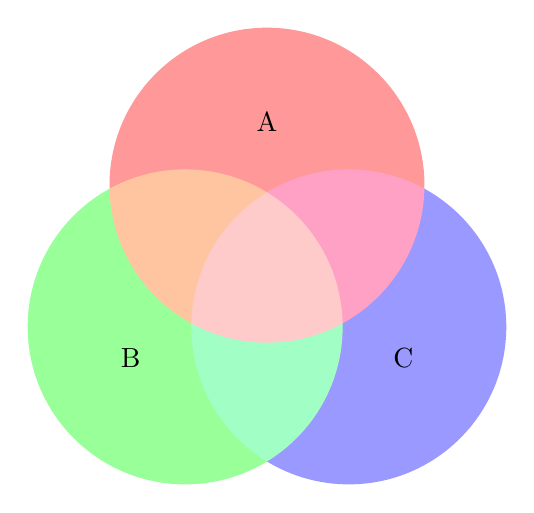
\begin{tikzpicture}

\begin{scope}[blend group=soft light]
\fill[red!40!white]
(90:1.2)  circle (2);
\fill[green!40!white]
(210:1.2) circle (2);
\fill[blue!40!white]
(330:1.2) circle (2);
\end{scope}

\node at (90:2)     {A};
\node at (210:2)    {B};
\node at (330:2)    {C};		

\end{tikzpicture}
\end{lstlisting}	
}

\end{minipage}
%%
%%
\begin{minipage}{.48\textwidth}

\scalebox{.8}{
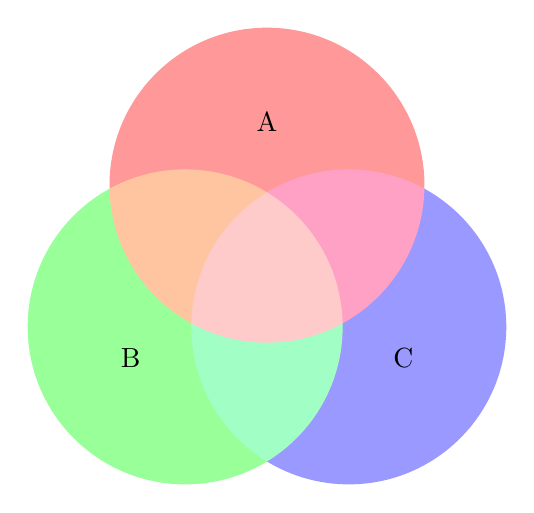
\begin{tikzpicture}
\begin{scope}[blend group=soft light]
\fill[red!40!white]   (90:1.2)  circle (2);
\fill[green!40!white] (210:1.2) circle (2);
\fill[blue!40!white]  (330:1.2) circle (2);
\end{scope}

\node at (90:2)    {A};
\node at (210:2)    {B};
\node at (330:2)    {C};		
\end{tikzpicture}	
}
\end{minipage}	

\end{frame}


%%%%%%%%%%%%%%%%%%%%%%%%%%%%%%%%%%

\begin{frame}[fragile]
%\frametitle{tikz-Beispiel}

\begin{minipage}{.62\textwidth}
{\tiny
\begin{lstlisting}	
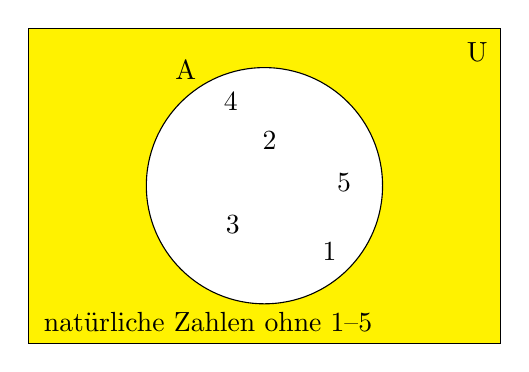
\begin{tikzpicture}
\def\firstrectangle{(0,0) rectangle (6,4)} 	
\def\firstcircle{(3,2) circle (1.5cm)}
\def\secondcircle{(0:2cm) circle (1.5cm)}

\begin{scope}[shift={(-3cm,2cm)}]
\clip \firstrectangle;
\fill[yellow] \firstrectangle;
\fill[white] \firstcircle;
\end{scope}

\begin{scope}[shift={(-3cm,2cm)}]
\draw \firstcircle;
\draw \firstrectangle;
\node at (33:6.8)   {U};
\node at (60:4)    {A};
\node at (40:4)    {2};
\node at (30:3)    {3};
\node at (17:4)    {1};
\node at (50:4)    {4};
\node at (27:4.5)  {5};
\node at (6.9:2.3) {natürliche Zahlen ohne 1--5};
\end{scope}
\end{tikzpicture}

\end{lstlisting}	
}

\end{minipage}
%%
%%
\begin{minipage}{.37\textwidth}
\scalebox{.7}{
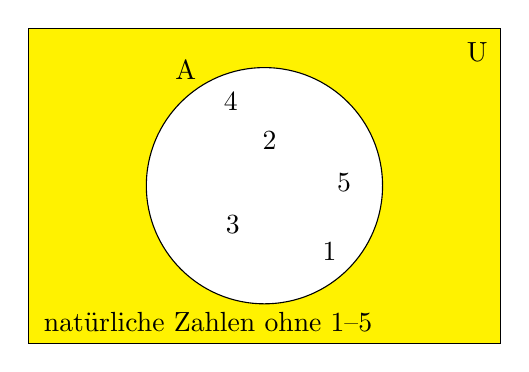
\begin{tikzpicture}

\def\firstrectangle{(0,0) rectangle (6,4)} 	
\def\firstcircle{(3,2) circle (1.5cm)}
\def\secondcircle{(0:2cm) circle (1.5cm)}

\begin{scope}[shift={(-3cm,2cm)}]
\clip \firstrectangle;
\fill[yellow] \firstrectangle;
\fill[white] \firstcircle;
\end{scope}

\begin{scope}[shift={(-3cm,2cm)}]
\draw \firstcircle;
\draw \firstrectangle;
\node at (33:6.8)    {U};
\node at (60:4)    {A};
\node at (40:4)    {2};
\node at (30:3)    {3};
\node at (17:4)    {1};
\node at (50:4)    {4};
\node at (27:4.5)  {5};
\node at (6.9:2.3)  {natürliche Zahlen ohne 1--5};

\end{scope}

\end{tikzpicture}
}
\end{minipage}	

\end{frame}


%%%%%%%%%%%%%%%%%%%%%%%%%%%%%%%%%%

\begin{frame}[fragile]
%\frametitle{tikz-Beispiel}

\begin{minipage}{.67\textwidth}
{\tiny
\begin{lstlisting}	
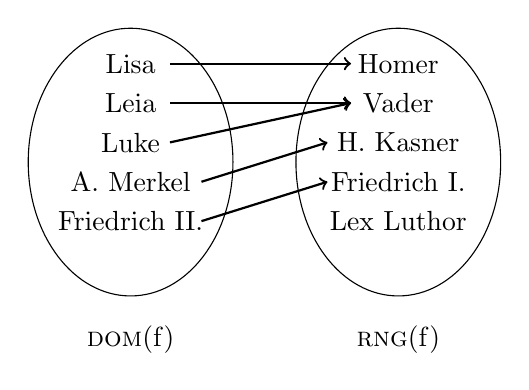
\begin{tikzpicture}
\def\firstellipse{(0,0) ellipse (1.3cm and 1.7cm)}
\def\secondellipse{(3.4,0) ellipse (1.3cm and 1.7cm)}
\begin{scope} 
\draw \firstellipse ;
\draw \secondellipse ;	
\node at (90:-2.25)  {\textsc{dom}(f)};
\node at (90:1.25)    {\blue{Lisa}}; 
\node at (90:.75)     {\blue{Leia}};
\node at (90:.25)     {\blue{Luke}};
\node at (90:-.25)    {\blue{A. Merkel}};
\node at (90:-.75)    {\blue{Friedrich II.}};
\node at (3.4,-2.25)  {\textsc{rng}(f)};			
\node at (3.4,1.25)    {\alert{Homer}}; 
\node at (3.4,.75)     {\alert{Vader}}; 
\node at (3.4,.25)     {\alert{H. Kasner}}; 
\node at (3.4,-.25)    {\alert{Friedrich I.}}; 
\node at (3.4,-.75)    {\alert{Lex Luthor}}; 
\draw[thick,->] (.5,1.25) -- (2.8,1.25);	
\draw[thick,->] (.5,.75)  -- (2.8,.75);	
\draw[thick,->] (.5,.25)  -- (2.8,.75);
\draw[thick,->] (.9,-.25) -- (2.5,.25);
\draw[thick,->] (.9,-.75) -- (2.5,-.25);
\end{scope}
\end{tikzpicture}
\end{lstlisting}	
}

\end{minipage}
%%
%%
\begin{minipage}{.32\textwidth}
\scalebox{.66}{
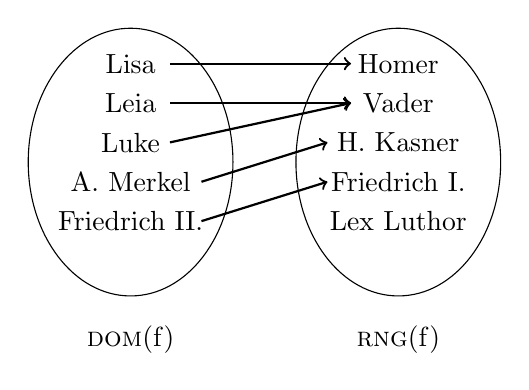
\begin{tikzpicture}

\def\firstellipse{(0,0) ellipse (1.3cm and 1.7cm)}
\def\secondellipse{(3.4,0) ellipse (1.3cm and 1.7cm)}

\begin{scope} 

\draw \firstellipse ;
\draw \secondellipse ;	

\node at (90:-2.25)  {\textsc{dom}(f)};
\node at (90:1.25)   {\blue{Lisa}}; 
\node at (90:.75)    {\blue{Leia}};
\node at (90:.25)    {\blue{Luke}};
\node at (90:-.25)   {\blue{A. Merkel}};
\node at (90:-.75)   {\blue{Friedrich II.}};


\node at (3.4,-2.25)  {\textsc{rng}(f)};			
\node at (3.4,1.25)   {\alert{Homer}}; 
\node at (3.4,.75)    {\alert{Vader}}; 
\node at (3.4,.25)    {\alert{H. Kasner}}; 
\node at (3.4,-.25)   {\alert{Friedrich I.}}; 
\node at (3.4,-.75)   {\alert{Lex Luthor}}; 


\draw[thick,->] (.5,1.25) -- (2.8,1.25);	
\draw[thick,->] (.5,.75)  -- (2.8,.75);	
\draw[thick,->] (.5,.25)  -- (2.8,.75);
\draw[thick,->] (.9,-.25) -- (2.5,.25);
\draw[thick,->] (.9,-.75) -- (2.5,-.25);

\end{scope}

\end{tikzpicture}
}
\end{minipage}	

\end{frame}


%%%%%%%%%%%%%%%%%%%%%%%%%%%%%%%%%%
%%%%%%%%%%%%%%%%%%%%%%%%%%%%%%%%%%
\subsection{Drawing with venndiagram}
%\frame{
%	\frametitle{~}
%	\begin{multicols}{2}
%		\tableofcontents[currentsection,hideallsubsections]
%	\end{multicols}
%}
%%%%%%%%%%%%%%%%%%%%%%%%%%%%%%%%%%
%%%%%%%%%%%%%%%%%%%%%%%%%%%%%%%%%%

\begin{frame}[fragile]
\frametitle{Drawing with venndiagram}

Load the package:

\begin{lstlisting}
\usepackage{venndiagram}
\end{lstlisting}


This package defines two environments:

\begin{enumerate}
	\item Venn diagrams with two sets
	\item Venn diagrams mwith three sets
\end{enumerate}

\begin{lstlisting}
\begin{venndiagram2sets}

\end{venndiagram2sets}
\end{lstlisting}

\begin{lstlisting}
\begin{venndiagram3sets}

\end{venndiagram3sets}
\end{lstlisting}

\end{frame}


%%%%%%%%%%%%%%%%%%%%%%%%%%%%%%%%%%
\begin{frame}[fragile]
%\frametitle{Venndiagramme zeichnen}


\begin{columns}

\begin{column}{.45\textwidth}

\begin{lstlisting}
\begin{venndiagram2sets}
\fillA \fillB
\end{venndiagram2sets}
\end{lstlisting}

\begin{venndiagram2sets}
	\fillA \fillB
\end{venndiagram2sets}

\end{column}
%%
%%
\begin{column}{.45\textwidth}

\begin{lstlisting}
\begin{venndiagram3sets}
\fillA \fillC
\end{venndiagram2sets}
\end{lstlisting}

\begin{venndiagram3sets}
	\fillA  \fillC
\end{venndiagram3sets}

\end{column}

\end{columns}

\end{frame}


%%%%%%%%%%%%%%%%%%%%%%%%%%%%%%%%%%
\begin{frame}[fragile]
%\frametitle{Venndiagramme zeichnen}


\begin{columns}

\begin{column}{.45\textwidth}

\begin{lstlisting}
\begin{venndiagram2sets}
\fillACapB
\end{venndiagram2sets}
\end{lstlisting}

\begin{venndiagram2sets}
\fillACapB
\end{venndiagram2sets}

\end{column}
%%
%%
\begin{column}{.45\textwidth}

\begin{lstlisting}
\begin{venndiagram3sets}
\fillOnlyC
\end{venndiagram2sets}
\end{lstlisting}

\begin{venndiagram3sets}
\fillOnlyC
\end{venndiagram3sets}

\end{column}

\end{columns}

\end{frame}


%%%%%%%%%%%%%%%%%%%%%%%%%%%%%%%%%%
\begin{frame}[fragile]
%\frametitle{Venndiagramme zeichnen}

\textbf{Elements} of the sets are given as options to the environment.

\begin{columns}

\begin{column}{.45\textwidth}
{\small
\begin{lstlisting}
\begin{venndiagram3sets}[
labelOnlyA={1},
labelOnlyB={2}, 
labelOnlyC={3}, 
labelOnlyAB={4}, 
labelOnlyAC={5}, 
labelOnlyBC={6}, 
labelABC={7},
labelNotABC={8}
]

\fillOnlyA
\end{venndiagram3sets}
\end{lstlisting}
}
\end{column}
%%
%%
\begin{column}{.45\textwidth}

\begin{venndiagram3sets}[labelOnlyA={1},labelOnlyB={2},labelOnlyC={3},
labelOnlyAB={4},labelOnlyAC={5},labelOnlyBC={6},labelABC={7},
labelNotABC={8}]

\fillOnlyA
\end{venndiagram3sets}

\end{column}

\end{columns}

\end{frame}

%%%%%%%%%%%%%%%%%%%%%%%%%%%%%%%%%%
%%%%%%%%%%%%%%%%%%%%%%%%%%%%%%%%%%
\subsection{Further features}
%\frame{
%	\frametitle{~}
%	\begin{multicols}{2}
%		\tableofcontents[currentsection,hideallsubsections]
%	\end{multicols}
%}
%%%%%%%%%%%%%%%%%%%%%%%%%%%%%%%%%%
%%%%%%%%%%%%%%%%%%%%%%%%%%%%%%%%%%

\begin{frame}[fragile]
\frametitle{Further features}

\begin{itemize}
\item For further features, check the package documentation \citep{Talbot16a}.

\item For complex diagrams, it is recommendable to use \ltxterm{TikZ}.
\end{itemize}

\end{frame}


%%%%%%%%%%%%%%%%%%%%%%%%%%%%%%%%%%
%%%%%%%%%%%%%%%%%%%%%%%%%%%%%%%%%%
\section{Vowel diagram}
\frame{
	\frametitle{~}
%	\begin{multicols}{2}
		\tableofcontents[currentsection,hideallsubsections]
%	\end{multicols}
}
%%%%%%%%%%%%%%%%%%%%%%%%%%%%%%%%%%
%%%%%%%%%%%%%%%%%%%%%%%%%%%%%%%%%%

\begin{frame}[fragile]
\frametitle{Vowel diagram}

Load the package \ltxpack{vowel} (it works with the package \ltxpack{tipa}):

\begin{lstlisting}
\usepackage{vowel}
\end{lstlisting}

\pause 
\bigskip

Vowel provides a \textbf{\ltxterm{vowel} environment} with different \textbf{options}:

\begin{columns}

\begin{column}{.40\textwidth}

\begin{lstlisting}
\begin{vowel}
\end{vowel}
\end{lstlisting}

\begin{figure}
	\centering	
	\begin{vowel}
	\end{vowel}
\end{figure}

\end{column}
%%
%%
\begin{column}{.5\textwidth}

\begin{lstlisting}
\begin{vowel}[triangle,three]
\end{vowel}
\end{lstlisting}

\begin{figure}
	\centering	
	\begin{vowel}[triangle,three]
	\end{vowel}
\end{figure}\end{column}

\end{columns}

\end{frame}


%%%%%%%%%%%%%%%%%%%%%%%%%%%%%%%%%%
%%%%%%%%%%%%%%%%%%%%%%%%%%%%%%%%%%
%\subsection{Vokale hinzufügen}
%\frame{
%	\frametitle{~}
%	\begin{multicols}{2}
%		\tableofcontents[currentsection,hideallsubsections]
%	\end{multicols}
%}
%%%%%%%%%%%%%%%%%%%%%%%%%%%%%%%%%%
%%%%%%%%%%%%%%%%%%%%%%%%%%%%%%%%%%

\begin{frame}[fragile]
%\frametitle{Vokale hinzufügen}

Vowels can be included with the command \lstinline|putcvowel|.

\begin{columns}

\begin{column}{.65\textwidth}

\begin{lstlisting}
\putcvowel[l|r]{x}{y}
\end{lstlisting}

\begin{itemize}
\item Options: \lstinline|l| or \lstinline|r| \ras left or right of a node \lstinline|y|

\item Arguments: 

\lstinline|x| \ras IPA symbol

\lstinline|y| \ras position in the diagram (every position in the diagram has a number!)

\end{itemize}

%\begin{lstlisting}
%\putvowel[l|r]{x}{z}{w}
%\end{lstlisting}

\end{column}
%%
%%
\begin{column}{.35\textwidth}


\begin{vowel}
\putcvowel{1}{1}
%	\putcvowel[r]{1}{1}
\putcvowel{2}{2}
%	\putcvowel[r]{2}{2}
\putcvowel{3}{3}
%	\putcvowel[r]{3}{3}
\putcvowel{4}{4}
%	\putcvowel[r]{4}{4}
\putcvowel{5}{5}
%	\putcvowel[r]{5}{5}
\putcvowel{6}{6}
%	\putcvowel[r]{6}{6}
\putcvowel{7}{7}
%	\putcvowel[r]{7}{7}
\putcvowel{8}{8}
%	\putcvowel[r]{8}{8}
\putcvowel{9}{9}
%	\putcvowel[r]{9}{9}
\putcvowel{10}{10}
%	\putcvowel[r]{10}{10}
\putcvowel{11}{11}
\putcvowel{12}{12}
%	\putcvowel[r]{12}{12}
\putcvowel{13}{13}
\putcvowel{14}{14}
\putcvowel{15}{15}
\putcvowel{16}{16}
\end{vowel}

\end{column}

\end{columns}



\begin{columns}

\begin{column}{.65\textwidth}
{\footnotesize
\begin{lstlisting}
\begin{vowel}
\putcvowel[l]{i}{1}
\putcvowel[l]{\textscripta}{5}
\putcvowel{\textschwa}{11}
\putcvowel{\textupsilon}{14}
\end{vowel}
\end{lstlisting}
}

\end{column}
%%
%%
\begin{column}{.35\textwidth}

\begin{vowel}
\putcvowel[l]{i}{1}
%	\putcvowel[r]{y}{1}
%	\putcvowel[l]{e}{2}
%	\putcvowel[r]{\o}{2}
%	\putcvowel[l]{\textepsilon}{3}
%	\putcvowel[r]{\oe}{3}
%	\putcvowel[l]{a}{4}
%	\putcvowel[r]{\textscoelig}{4}
%	\putcvowel[l]{\textscripta}{5}
\putcvowel[r]{\textturnscripta}{5}
%	\putcvowel[l]{\textturnv}{6}
%	\putcvowel[r]{\textopeno}{6}
%	\putcvowel[l]{\textramshorns}{7}
%	\putcvowel[r]{o}{7}
%	\putcvowel[l]{\textturnm}{8}
%	\putcvowel[r]{u}{8}
%	\putcvowel[l]{\textbari}{9}
%	\putcvowel[r]{\textbaru}{9}
%	\putcvowel[l]{\textreve}{10}
%	\putcvowel[r]{\textbaro}{10}
\putcvowel{\textschwa}{11}
%	\putcvowel[l]{\textrevepsilon}{12}
%	\putcvowel[r]{\textcloserevepsilon}{12}
%	\putcvowel{\textsci\ \textscy}{13}
\putcvowel{\textupsilon}{14}
%	\putcvowel{\textturna}{15}
%	\putcvowel{\ae}{16}
\end{vowel}

\end{column}

\end{columns}

\end{frame}


%%%%%%%%%%%%%%%%%%%%%%%%%%%%%%%%%%
\begin{frame}[fragile]
%\frametitle{Vokale hinzufügen}

Vowels can be included with the command \lstinline|putvowel|.

\begin{lstlisting}
\putvowel[l|r]{x}{z}{w}
\end{lstlisting}

\begin{itemize}
\item Options:  \lstinline|l| or \lstinline|r| \ras left or right of a node \lstinline|y|

\item Arguments: 

\lstinline|x| \ras IPA symbol

\lstinline|z| \ras coordinate on x axis

\lstinline|w| \ras coordinate on y axis
\end{itemize}


\begin{columns}

\begin{column}{.65\textwidth}
{\footnotesize
\begin{lstlisting}
\begin{vowel}
\putvowel[l]{i}{0pt}{0pt}
\putvowel[r]{y}{0pt}{0pt}
\putvowel{a}{42pt}{66pt}
\putvowel{u}{99pt}{0pt}
\end{vowel}
\end{lstlisting}
}

\end{column}
%%
%%
\begin{column}{.35\textwidth}

\begin{vowel}
\putvowel[l]{i}{0pt}{0pt}
\putvowel[r]{y}{0pt}{0pt}
%	\putvowel{i}{0pt}{0pt}
\putvowel{a}{42pt}{66pt}
\putvowel{u}{99pt}{0pt}
\end{vowel}

\end{column}

\end{columns}

\end{frame}


%%%%%%%%%%%%%%%%%%%%%%%%%%%%%%%%%%
\begin{frame}[fragile]
%\frametitle{Vokale hinzufügen}

\begin{multicols}{2}
	
\begin{lstlisting}
\begin{vowel}
\putcvowel[l]{i}{1}
\putcvowel[r]{y}{1}
\putcvowel[l]{e}{2}
\putcvowel[r]{\o}{2}
\putcvowel[l]{\textepsilon}{3}
\putcvowel[r]{\oe}{3}
\putcvowel[l]{a}{4}
\putcvowel[r]{\textscoelig}{4}
\putcvowel[l]{\textscripta}{5}
\putcvowel[r]{\textturnscripta}{5}
\putcvowel[l]{\textturnv}{6}
\putcvowel[r]{\textopeno}{6}
\putcvowel[l]{\textramshorns}{7}
\putcvowel[r]{o}{7}
\putcvowel[l]{\textturnm}{8}
\putcvowel[r]{u}{8}
\putcvowel[l]{\textbari}{9}
\putcvowel[r]{\textbaru}{9}
\putcvowel[l]{\textreve}{10}
\putcvowel[r]{\textbaro}{10}
\putcvowel{\textschwa}{11}
\putcvowel[l]{\textrevepsilon}{12}
\putcvowel[r]{\textcloserevepsilon}{12}
\putcvowel{\textsci\ \textscy}{13}
\putcvowel{\textupsilon}{14}
\putcvowel{\textturna}{15}
\putcvowel{\ae}{16}
\end{vowel}
\end{lstlisting}

\begin{figure}
\centering
{\Large
\begin{vowel}
\putcvowel[l]{i}{1}
\putcvowel[r]{y}{1}
\putcvowel[l]{e}{2}
\putcvowel[r]{\o}{2}
\putcvowel[l]{\textepsilon}{3}
\putcvowel[r]{\oe}{3}
\putcvowel[l]{a}{4}
\putcvowel[r]{\textscoelig}{4}
\putcvowel[l]{\textscripta}{5}
\putcvowel[r]{\textturnscripta}{5}
\putcvowel[l]{\textturnv}{6}
\putcvowel[r]{\textopeno}{6}
\putcvowel[l]{\textramshorns}{7}
\putcvowel[r]{o}{7}
\putcvowel[l]{\textturnm}{8}
\putcvowel[r]{u}{8}
\putcvowel[l]{\textbari}{9}
\putcvowel[r]{\textbaru}{9}
\putcvowel[l]{\textreve}{10}
\putcvowel[r]{\textbaro}{10}
\putcvowel{\textschwa}{11}
\putcvowel[l]{\textrevepsilon}{12}
\putcvowel[r]{\textcloserevepsilon}{12}
\putcvowel{\textsci\ \textscy}{13}
\putcvowel{\textupsilon}{14}
\putcvowel{\textturna}{15}
\putcvowel{\ae}{16}
\end{vowel}
}
\end{figure}
\end{multicols}


\end{frame}




%%%%%%%%%%%%%%%%%%%%%%%%%%%%%%%%%%
%%%%%%%%%%%%%%%%%%%%%%%%%%%%%%%%%%
\subsection{Further features}
%\frame{
%	\frametitle{~}
%	\begin{multicols}{2}
%		\tableofcontents[currentsection,hideallsubsections]
%	\end{multicols}
%}
%%%%%%%%%%%%%%%%%%%%%%%%%%%%%%%%%%
%%%%%%%%%%%%%%%%%%%%%%%%%%%%%%%%%%

\begin{frame}[fragile]
\frametitle{Further features}

Check the documentation \citep{Rei01a} for more features.

\bigskip


Check also Felix Kopecky's solution (for Language Science Press) with \ltxterm{TikZ}:\\
\url{http://userblogs.fu-berlin.de/langsci-press/2016/06/15/drawing-vowel-charts-with-tikz/}

\end{frame}


%%%%%%%%%%%%%%%%%%%%%%%%%%%%%%%%%%
%\begin{frame}[fragile]
%\frametitle{Exercise}
%
%
%Go to \url{https://github.com/langsci/latex4linguists/blob/master/4-1.md}\\
%and\\
%\url{https://github.com/langsci/latex4linguists/blob/master/4-2.md}
%and follow the instructions of \textbf{all blocks} in your \texttt{.tex} file.
%
%%Download the PDF \alert{\texttt{myDocument-EX4.pdf}} and replicate it with the commands you have already learnt. Follow the instructions in the last section and install the packages.
%
%\end{frame}


%%%%%%%%%%%%%%%%%%%%%%%%%%%%%%%%%%%
%%%%%%%%%%%%%%%%%%%%%%%%%%%%%%%%%%%
%\section{XY}
%%\frame{
%%\begin{multicols}{2}
%%\frametitle{~}
%%	\tableofcontents[currentsection]
%%\end{multicols}
%%}
%%%%%%%%%%%%%%%%%%%%%%%%%%%%%%%%%%%
%
%\begin{frame}{XY}
%
%\begin{itemize}
%	\item XY
%\end{itemize}
%
%\end{frame}


%%%%%%%%%%%%%%%%%%%%%%%%%%%%%%%%%%%%
%%%%%%%%%%%%%%%%%%%%%%%%%%%%%%%%%%%%
%\iftoggle{handout}{
%%% BEGIN handout true
%
%%%%%%%%%%%%%%%%%%%%%%%%%%%%%%%%%%%%
%	
%%Test Toggle ON
%
%}
%%% END handout true 
%%% BEGIN handout false
%{
%%%%%%%%%%%%%%%%%%%%%%%%%%%%%%%%%%%%
%
%% Test Toggle OFF
%
%}%% END handout false
%%%%%%%%%%%%%%%%%%%%%%%%%%%%%%%%%%%%